\documentclass{article}
\usepackage[utf8]{inputenc}
\usepackage{wrapfig}
\usepackage{natbib}
\usepackage{graphicx}

\begin{document}

\section{One water tank system}

\subsection{Process description}

Consider the water tank system as shown in the fig.~\ref{Tank_Schema}.
This system consists of the water tank with cross-sectional area $A_t$ and height $H$,
orifice with cross-sectional area $A_{out}$, level sensor, pumping unit $P$, 
controller $C$ and water basin.

\begin{figure}[ht]
\centering
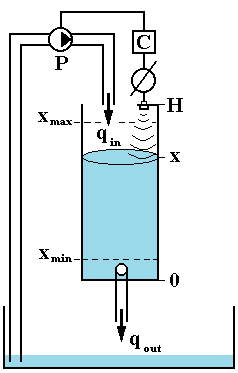
\includegraphics[width=0.4\textwidth]{Pic/wt_s.png}
\caption{Water tank system}
\label{Tank_Schema}
\end{figure}

In this setup the pump provides in-feed of the water $q_{in}$ to the tank from the basin.
The outflow $q_{out}$ of the tank is emptied the water back.


\subsection{Controller requirements}
The following conditions with regard to the system are used to describe the level of the water $x$ in the tank:
\begin{itemize}
\item The level of the water is measured by sensor.
\item The controller is able to force on the pumping unit by changing the voltage $u$ applied to the input terminals of the pump (see fig.~\ref{Control_Diag}).
\end{itemize}

\begin{figure}[ht]
\centering
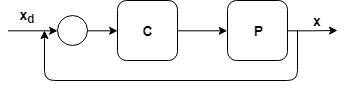
\includegraphics[width=0.35\textwidth]{Pic/wt_cd.png}
\caption{Control diagram}
\label{Control_Diag}
\end{figure}

\begin{itemize}
\item In nominal conditions controller allows to keep desired level of the water $x_d$ in a predicted domain $[x_{min}, x_{max}]$.
\item Controller is capable to handle the situation of low level protection ($0 < x < x_{min}$) as well as the situation of the high level protection  ($x_{min} < x < H$).
\item Controller should also avoid the situation of overflow (see fig.~\ref{State_Diag}).
\end{itemize}

\begin{figure}[ht]
\centering
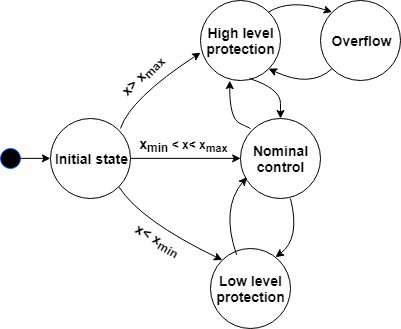
\includegraphics[width=0.45\textwidth]{Pic/wt_st.png}
\caption{State diagram}
\label{State_Diag}
\end{figure}

As a direct sequence we can formulate the list of the requirements for a controller:
\begin{enumerate}
	%% spaces \ \, \;
	\item  {$G\ (x_d   \in  [\, x_{min}\, , \, x_{max} \,])$. The desired water level always lies in a given interval. }
	\item  {$G!\ (du/dt \leq D_{min})$. The control signal always changes smoothly.}
	\item  {$G!\ (x \leq 0)$. The water level is always  greater than zero.}
	\item  {$G\ (u   \in  [\, u_{min} \, , \,  u_{max} \, ])$. The control signal always lies in a given interval.}
\end{enumerate}

\textbf{\citep{simulator}!!! Do not forget about cites!}

Let $x$ be a measured water level in the water tank and simultaneously the input parameter for the controller.
Then, based on the assumptions above, the dynamic equation for the water level is derived as follows. 
For the tank the rate pf change of the water level in a time is given by
\begin{equation}
\label{Eq_x_dot_source}
\dot{x}(t)=\frac{1}{A_t}(q_{in}(t)-q_{out}(t))~~~\left [ \frac{cm}{sec} \right ],
\end{equation}
where $x$, $A_t$,$q_in$, $q_out$ are the water level, cross-sectional area of the tank, inflow rate, outflow rate respectively. Next, note that the inflow rate to the tank is given by
\begin{equation}
\label{Eq_q_in}
q_{in}(t)=K_p\cdot u_p(t)~~~\left [ \frac{cm^3}{sec} \right ],
\end{equation}
where $K_p$ is the pump constant $\left [ \frac{cm^3}{Volt \cdot sec} \right ]$ and the $u_p(t)$ is the voltage applied to the pump, the output parameter of the controller.
In addition, using the Torricelli's law for a flow through a small orifices, the outflow rate of the water from the tank is given by
\begin{equation}
\label{Eq_q_out}
q_{out}(t)=A_{out}\cdot\sqrt{2gx(t)}~~~\left [ \frac{cm^3}{sec} \right ],
\end{equation}
where $g$ is the gravitational acceleration, $A_{out}$ denotes the cross-sectional area of the outflow orifice at the bottom of the tank.

Using the (\ref{Eq_x_dot_source}--\ref{Eq_q_out}), we obtain the dynamic equation for the water level in the tank as
\begin{equation}
\label{Eq_x_dot}
\dot{x}(t)=\frac{1}{A_t}(K_p\cdot u_p(t)-A_{out}\cdot\sqrt{2gx(t)}).
\end{equation}

Note that using  (\ref{Eq_x_dot}), we can compute the steady-state pump voltage $u_p^{ss}$ that produces the desired steady-state level $x_d^{ss}$ in the tank. 
Specifically, setting the $\dot{x}(t)=0$ in (\ref{Eq_x_dot}) yields
\begin{equation}
\label{Eq_upss}
u_p^{ss}=A_{out} \cdot \frac{\sqrt{2g x_d^{ss}}}{K_p}.
\end{equation}

\section{Implementation in C\texttt{\#}}


\bibliographystyle{plain}
\bibliography{references}
\end{document}
